\documentclass{polytech/polytech}

\typereport{prddi5}

\reportyear{2017-2018}
\title{Plateforme d'acquisition et de formatage temps réel multiflux TV Web}
\student[di5]{Romain}{ROUSSEAU}{romain.rousseau@etu.univ-tours.fr}
\academicsupervisor[di]{Mathieu}{DELALANDRE}{mathieu.delalandre@univ-tours.fr}


\resume{Ce projet consiste en l'élaboration d'une plateforme d'acquisition de flux TV Web en temps réel. L'objectif dans un premier temps consistera en l'affichage de plusieurs flux en simultané avant d'éventuellement faire évoluer l'application pour y faire figurer des éléments d'analyse d'images. Au travers de ce rapport, nous verrons la démarche, les objectifs liés à la mise en place d'une telle plateforme, l'architecture logicielle avec une structure en multi-threads, ainsi qu'un état de l'art sur ce domaine constante expansion et qui représente près de 80\% du trafic de données sur Internet.}

\motcle{Plateforme d'acquisition} 
\motcle{Flux de données} 
\motcle{Temps réel}
\motcle{Protocole de communication} 
\motcle{Télévision en ligne}


\abstract{This project consists in the making of acquisition platform of Live TV streams in real time. The first aim is to display multiple streams at the same time before evolving the platform to add elements of frame analysis. Through this document, we will see the approach, the goals link in the making of such a platform, the software architecture with a multi-threaded structure, as a state-of-the-art in this constantly evolving domain which represents almost 80\% of data traffic on the Internet.}

\keyword{Streaming Platform}
\keyword{Live Stream}
\keyword{Real Time}
\keyword{Communication Protocol}
\keyword{Online TV}


\posterblock{Contexte}{Le domaine du streaming est en constante évolution et représente près de 80\% de trafic de données sur le net.
	
	Alors qu’il existe de nombreux outils pour analyser les vidéos hors-ligne, il en existe très peu pour analyser les flux en direct, ce qui pourrait apporter de nouvelles possibilités dans de nombreux domaines du secteur des médias.}{images/illuStreaming}{Illustration sur le streaming}

\posterblock{Objectifs}{Le but est de réaliser une plateforme d’acquisition multi-flux TV Web. Dans un premier temps, le souhait est d’afficher en simultané plusieurs flux TV par le biais de la plateforme.
	
	Par la suite, nous pourrons implémenter des éléments de statistiques sur le flux arrivant ou bien de l’analyse d’images}{images/streamlink}{Aperçu de l'invite de commande pour le lancement de la plate-forme}

\posterblock{Fonctionnalités}{
	\begin{itemize}
		\item Sélection des chaînes désirées sur un fichier texte;
		\item Lancement de la plate-forme en ligne de commande;
		\item Affichage des flux en simultanés, avec gestion de la synchronisation.
	\end{itemize}
}{images/affichageFlux}{Exemple d'affichage de plusieurs chaînes en simultané}



\addbibresource{biblio.bib}

%%%%%%%%%%%%%%%%%%%%%%%%%%%%%%%%%%%%%%%%%%%%%%%%%%%%%%%%%%%%%%%%%%%%%%%%%%%%%%%%%%%%%%%%%%%%%%%%%%%
%%%%%%%%%%%%%%%%%%%%%%%%%%%%%%%%%%%%%%%%%%%%%%%%%%%%%%%%%%%%%%%%%%%%%%%%%%%%%%%%%%%%%%%%%%%%%%%%%%%

\begin{document}


\chapter*{Introduction}


Alors qu’approche la fin du cursus à l’école Polytech Tours, se dresse le projet le plus important du parcours, le projet Recherche et Développement. Il s’étale sur l’ensemble de la cinquième année et représente une forme de synthèse des connaissances acquises lors des années d’études précédentes. Il permet de développer et d’approfondir son savoir sur un ou plusieurs champs de compétences spécifiques, afin de devenir un spécialiste du domaine choisi dans le cadre du projet. Ce projet est mené seul, sous la supervision du tuteur académique et avec l’aide d’un intervenant extérieur qui fait partie des initiateurs du sujet. Il permet ainsi de développer son autonomie en menant à bien un travail des prémices jusque, dans le meilleur des cas, à la production.

J’ai décidé de me consacrer à un sujet lié à un domaine en plein essor : le streaming. Ce sujet faisait partie de mes choix privilégiés lorsque j’ai vu la liste des sujets proposés. En effet, je regarde moi-même beaucoup de contenu audiovisuel par ce biais. J’ai pris pour habitude de regarder mes programmes télévisuelles préférés via mon ordinateur plutôt que par les usages traditionnelles avec une télévision depuis plusieurs années déjà, et il m’a paru intéressant de me pencher sur l’envers du décor et le fonctionnement de ces applications utilisées au quotidien par des milliers de personnes aujourd’hui.

Le but du projet est de réaliser une plateforme pour l’acquisition de flux de TV Web. Le contexte, les acteurs et les objectifs seront détaillés dans la première partie de ce rapport. En deuxième partie, nous retrouverons l’état de l’art et la veille technologique pour la plateforme, à savoir des informations sur les protocoles utilisés, les différentes librairies d’acquisition, les serveurs distribuant les flux, etc. La description générale du projet, avec son environnement, ses fonctionnalités et ses caractéristiques, sera dans la troisième partie de ce rapport. Le choix de présenter l’état de l’art et la veille technologique avant la description de la plateforme découle de la présentation des librairies et des protocoles utilisés, détaillés dans la deuxième partie. Il s’agit d’un choix qui permet d’accroître sa compréhension lorsque les descriptions fonctionnelles seront présentées. Enfin nous évoquerons les prémices d’analyse et de conception de la plateforme dans la dernière partie.

Des éléments complémentaires concernant notamment la gestion de projet via un diagramme
de Gantt sont disponibles en annexes.



\part{Contexte de la réalisation et cadre générale du projet}


Cette partie est consacrée à la description du cadre général du projet, c’est-à-dire ce pourquoi le sujet a été proposé, qui sont les acteurs autour de celui-ci, les enjeux posés, etc.


\section{Contexte, enjeux et acteurs}


Aujourd’hui, Internet est l’un des supports les plus répandus pour échanger et partager de l’information. En constante expansion, Internet est accessible par plus de la moitié de la population mondiale \cite{_chiffres_2017}. L’un des aspects majeurs d’Internet est la diffusion de contenu audio et vidéo, en effet plus de 75\% du trafic actuel est constitué de données vidéo et ce pourcentage augmentera jusqu’à plus de 80\% à l’horizon 2021 \cite{_cisco_2017}. La demande continue de prendre de l’ampleur au fil des années, les consommateurs demandant des vidéos avec la meilleure qualité possible.

Avec cette évolution constante, la diffusion de contenu vidéo en ligne est devenue un enjeu majeur pour les entreprises s’installant sur Internet et en particulier pour celles spécialisées dans l’audio-visuel et les médias. Les plus grands groupes ont déjà tous développé des services permettant de voir leurs programmes en direct ou en différé sur Internet depuis plusieurs années déjà. Aujourd’hui, elles sont utilisées couramment par le grand public (exemple avec la plateforme MyCanal du groupe Canal + qui compte 5 millions de visiteurs uniques par mois et près de 2 millions d’utilisateurs actifs \cite{sancerre_canal+_2017}) et les principaux acteurs du secteur tendent à vouloir élargir leur offre en se démarquant du modèle de la télévision traditionnelle.


\begin{figure}
	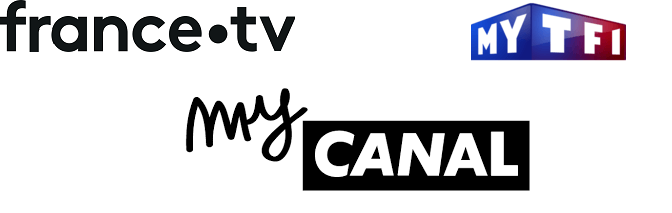
\includegraphics[scale=0.75]{images/exemple_sites.png}
	\caption{Exemples de plate-forme vidéo de grands groupes audio-visuels français}
	\label{fig:ex_plate-formes}
\end{figure}

Ils existent déjà de nombreux outils pour acquérir, stocker, traiter et indexer les flux de Web TV hors-ligne \cite{abduraman_tv_2012}. Cependant, la tendance actuelle est l’analyse de ces flux en continu, notamment par le biais de la détection de vidéos dupliquées \cite{liu_near-duplicate_2013}. Ce type d’analyse peut être appliqué à de nombreux domaines faisant l’objet d’enjeux majeurs pour les entreprises du secteur comme la protection de la propriété intellectuelle, la recommandation de vidéo, ou même le contrôle des vidéos.


Prenons un exemple d’analyse en continu qui est susceptible d’être utilisé dans le cadre de la télévision sur le web. Une entreprise souhaite vérifier si ces publicités sont bien passées à l’antenne. Par le biais de la détection vidéo, il serait possible en analysant le flux d’une chaîne souhaitée de savoir si la publicité est bien passée, à quel moment de la journée, sa fréquence sur un temps donné, et d’autres données pouvant intéresser l’entreprise. Récupérer ces informations avec une analyse manuelle du chaîne est laborieuse et coûteuse.

Ce projet a été initié par un ancien étudiant de Polytech Tours, M. Jordan NICOT qui, pour son projet libre lors de son dernier semestre, a réalisé un programme de traitement d’un flux RTSP. L’idée derrière son projet était de détecter si une chaîne de télévision diffusait des publicités ou non. Pour cela, la plateforme prenait un flux RTSP venant de son boîtier TV et effectuait un traitement d’images détecter l’apparition du jingle de publicité de la chaîne analysée. Le traitement était assez rudimentaire, puisqu’il consistait en l’analyse d’un encart de l’image dans lequel était écrit, avec une typographie particulière, le mot "publicités". L’analyse fonctionnait bien pour une à deux chaînes, mais pas pour toutes. Cependant, l’idée principale a été conservée, et sera exploitée lors de ce projet.


\section{Objectifs}

L’objectif de ce projet est, à terme, de mettre en place une plateforme d’acquisition et de formatage en temps réel de flux TV Web. Le but est que cette plateforme soit adaptable afin que des éléments d’analyse et de traitements des données puissent être ajoutée par la suite. Pour le moment, nous nous contenterons d’afficher un ou plusieurs flux à l’écran en prenant en compte les capacités réseaux, et garantissant une synchronisation en horodatage des flux. Le projet s’appuiera sur une partie des travaux de Jordan NICOT lors de son projet libre de l’année dernière. Le code ne sera pas repris dans son intégralité, le programme final de ce projet sera seulement inspiré de ses travaux, notamment de gestion et d’affichage du flux. 

Ce sujet s’inscrit dans le cadre d’un projet de création de startup ImageStream engagé au niveau du Laboratoire d’Informatique Fondamentale de Tours (LIFAT), entre l’Université et le secteur privé. Ainsi, la plateforme pourra être réutilisée et amélioré si le projet abouti. Par ailleurs, pour ces raisons de création de Start-Up en lien avec l’Université, les tests de la plateforme seront réalisés via le réseau et les machines de l’université.

\section{Hypothèses}

Le but de l’application est d’acquérir des flux TV retransmis sur le Web. Cependant, avec l’évolution des protocoles de streaming (voir \autoref{chap:diffusion_flux}), il devient de plus en plus compliqué de récupérer un flux TV pour un programme tiers. Les grandes plateformes d’hébergement de flux nécessitent souvent d’avoir un compte sur le site en question ou d’être abonné à un fournisseur de services. L’un des intérêts de l’application est qu’elle fonctionne pour toutes les chaînes accessibles gratuitement sur la télévision française par la TNT. Or, certaines d’entre elles pourraient être difficiles d’accès pour la plateforme.

S’il n’est pas possible de récupérer les flux, de façon sûr et légal, alors nous effectuerons les tests uniquement sur des chaînes facilement accessibles, quelles soient françaises ou étrangères, comme par exemple : FranceInfo ou France24, toutes les deux disponibles sur Youtube.


\section{Base méthodologique}

Ce projet suivra une structure traditionnelle de cycle en V. En effet, elle est plus adaptée dans notre cas qu’une méthode Agile. La plateforme ne nécessite pas une grande réactivité dans les demandes clients et n’a besoin de fonctionnement sous forme de sprint pour être réalisé. Étant donné qu’il n’y a pas de clients pour le moment, les demandes sont déjà connues et ne sont pas amenées à évoluer pour ce qui est de la partie Analyse des besoins.


De plus, certaines étapes du cycle ont déjà été réalisé, la partie Analyse des besoins notamment, ainsi que la partie concernant les spécifications fonctionnelles. Le détail de la gestion de ce projet sont disponibles en annexes, avec le diagramme de Gantt. Il est à noter que ce diagramme est uniquement à but informatif, et les dates limites des tâches présentes sur celui-ci sont susceptibles d’être modifiées au cours de l’avancement du projet.

Concernant le développement, nous suivrons une structure de type MVC (Modèle Vue Contrôleur) avec la partie Modèle qui se focalisera sur les objets Flux que nous allons créer, la partie Vue qui se concentrera sur l’affichage des fenêtres et sur l’interface en général et la partie Contrôleur qui fera la liaison entre les parties.



\part{\'{E}tat de l'art et Veille technologique}


\chapter{\'{E}tat de l'art sur la télévision}

\section{Diffusion d'une chaîne de télévision}

\section{Réception de la télévision}

\subsection{Réception Hertzienne}

\subsection{Réception par satellite}

\subsection{Réception par câble}

\subsection{Service par contournement ou Over the Top (OTT)}


\chapter{La diffusion de flux en continu sur Internet}
\label{chap:diffusion_flux}

Dans la partie suivante, nous allons effectuer un tour d’horizon sur les flux en continu diffusés sur Internet ainsi que sur les possibilités actuelles en terme d’exploitation de données. Nous répondrons par la suite à plusieurs problématiques : comment les flux en continu ont émergé avec le développement d’Internet ? Quels sont les protocoles existants permettant de transmettre ces flux de données? Quelles librairies nous permettent d’acquérir et d’exploiter ces flux? Autant de questions auxquelles nous allons nous pencher dans les pages qui suivent.

Une parenthèse cependant concernant la suite de ce rapport, nous emploierons plusieurs termes pour définir la même notion, à savoir les flux de données en continu. Nous les nommerons flux, flux TV Web ou encore Streaming ou Streaming vidéo indifféremment. Le terme Streaming est tiré de l’anglais stream signifiant flot ou courant en français. Ce terme désigne aujourd’hui dans le langage courant la diffusion en continu sur Internet de contenus audio-visuels. Il existe différents types de données que l’on peut diffuser en continu sur une plateforme, mais nous nous focaliserons essentiellement sur les flux vidéo en continu, qui sont les bases de ce projet. Nous pouvons noter que les autres principes de flux de données comme le streaming audio que l’on peut retrouver sur des plateformes comme Spotify ou Deezer fonctionnent sur des bases similaires. Seules les données transférées diffèrent.

\section{Principe générale du \textit{streaming}}

La diffusion de flux en continu repose sur le principe d’une communication entre un client et un serveur. Les données sont mis à disposition sur un serveur et pour récupérer ses informations, le client envoie une requête qui lui communique les données souhaitées. Il existe deux types de lectures distincts \cite{_definition_2017} :

\begin{description}
	\item[Lecture Progressive] Cette forme de lecture est celle que l’on retrouve lorsque l’on regarde une vidéo sur un navigateur par exemple. Ici la vidéo est chargée, les données sont mises en cache par le client et la vidéo commence lorsqu’il y a assez de données en cache pour la commencer. La plupart du temps, le serveur propose plusieurs versions du même fichier avec des qualités différentes pour pouvoir s’adapter à la bande passante du client. C’est le principe que l’on retrouve pour le visionnage de vidéos Youtube par exemple.
	\item[Lecture en continu] Il s’agit de la forme de lecture qui nous intéresse pour ce projet. Ici, le contenu est diffusé au même rythme que la lecture. L’une des différences majeures est que le fichier envoyé par le serveur n’a pas de début et de fin définis comme pour un fichier statique. C’est un flot de données qui est envoyé au fur et à mesure au client.
\end{description}

Pour notre projet, nous nous intéresserons uniquement à la lecture en continu, qui est le principe des flux TV sur le Web. Et en particulier, l’un des aspects que nous rechercherons par la suite sur la diffusion de flux est le \textit{streaming} adapté ou \textit{Adaptive Streaming} en anglais que nous détaillerons dans la \autoref{sec:adaptative_streaming}.



\section{Genèse du \textit{streaming} vidéo et évolution au fil du temps}

Dans les années 1990, Internet commence à se démocratiser. Il est désormais accessible de s’acheter un ordinateur personnel pour un foyer lambda, quand les prix étaient encore très élevés dans les années 1980. L’élargissement de la bande passante ainsi que l’amélioration de l’accès aux réseaux accélèrent le développement d’Internet tel qu’on le connaît aujourd'hui. La possibilité de communiquer entre différents foyers et de diffuser des informations à travers le monde devient de plus en plus accessible par le biais de ce jeune Internet.

C’est en 1995 qu’apparaît la première diffusion audio en ligne en continu sur Internet. Il s’agissait d’un match de baseball proposé aux abonnés d’\textit{ESPNSportZone} en ligne. Ainsi, les abonnés de partout dans le monde ont pu suivre le match via un enregistrement radiophonique \cite{zambelli_history_2013}. La diffusion a été mise en place par une entreprise du nom de Progressive Network, qui plus tard, est devenu \textit{Real Network}.

Par la suite, les grands groupes informatiques de l’époque ont déployé tour à tour leurs solutions. Au début des années 2000, trois plateformes ont le monopole du streaming : \textit{Real Player} de \textit{Real Network}, \textit{Windows Media Player} de \textit{Microsoft} et \textit{Quicktime Player} de \textit{Apple}, avec chacun leurs propres technologies et protocoles de communication. Nous verrons par ailleurs le détail de certains de ces protocoles dans la \autoref{sec:protocoles}.

\begin{figure}
	
\includegraphics[scale=0.70]{images/logos_platform.png}
	\caption{Exemples de plate-forme populaire dans les années 2000}
	\label{fig:logoPlatform}
\end{figure}

Au fil des années, la concurrence évolue et devient de plus en plus rude. La technologie s’améliore et les anciennes plateformes dominantes deviennent rapidement obsolètes. Arrive au courant des années 2000 Adobe et sa technologie Adode Flash qui s’impose rapidement dans tous les foyers, si bien que l’add-on Flash Player était installé sur 99\% des ordinateurs américains jusqu’en 2011 \cite{_chronique_streaming_2010}. Aujourd’hui, Flash Player est devenu obsolète pour plusieurs raisons : tout d’abord, la technologie entraînait de nombreux bugs et failles de sécurité que déploraient la plupart des services l’utilisant, et ensuite, l’avènement de l’HTML5 sur les navigateurs a permis d’incruster une vidéo sur une page web sans avoir besoin de plug-ins particuliers. Tous ces problèmes concernant Flash ont été listés notamment par Steve Jobs en personne en 2010 [WWW15], prônant par la même occasion le HTML5 et les nouvelles technologies émergentes. La page Flash sera définitivement tournée dans les années qui viennent, avec l’annonce d’Adobe le 25 juillet 2017 qui prévoit son abandon définitif à l’horizon 2020 [WWW5].

La tendance aujourd’hui est aux nouveaux protocoles qui fonctionnent indépendamment de toutes installations de plug-ins ou de programmes pour fonctionner. C’est le cas par exemple du protocole HLS que nous observerons plus en détails dans la \textit{subsec:newProto}. Par ailleurs, l’un des aspects importants de la diffusion en continu aujourd’hui est l’\textit{Adaptive Streaming} qui est exposé dans la partie suivante.

\section{Diffusion en flux adaptatif ou Adaptative Streaming}
\label{sec:adaptative_streaming}

\section{Les protocoles}
\label{sec:protocoles}

\subsection{HTTP}

\subsection{RTSP et RTSP 2.0}

\subsection{RTMP}

\subsection{MPEG-DASH, HLS, HDS et les nouveaux protocoles basés sur HTTP}
\label{subsec:newProto}


\section{Les formats de fichiers utilisés}


\chapter{Les chaînes de TV sur Internet en France}


\section{Critères de recherche}


\section{Résultats de l'étude}


\section{Tendances observées}


\section{Un mot sur le copyright}


\chapter{Les bibliothèques et logiciels d'acquisition}


\section{Les frameworks Windows (VfW, DirectShow, Media Foundation)}

\section{FFMPEG}


\section{libVLC et VLCJ}


\section{Streamlink}


\part{Description générale et analyse}


\chapter{Description générale}


\section{Environnement du projet}

\section{Caractéristiques des utilisateurs}


\section{Fonctionnalités du système}


\subsection{Séléction des chaînes via le fichier texte}

\subsection{Lancement en ligne de commande}

\subsection{Affichage des streams}

\section{Structure générale du système}


\subsection{La classe TVChannel}

\subsection{La classe MainLaunch}

\subsection{La classe MainControler}

\subsection{La classe StreamControler}

\subsection{La classe TextInputStreamControler}

\subsection{La classe StreamView}


\subsection{Lien entre les classes}


\chapter{Analyse des méthodes}



\part{Qualité de code et Tests de charges}


\chapter{Documentation et contrôle de qualité du code}


\section{Javadoc}


\section{Utilisation de SonarQube et SonarLint}

Pour le développement du site, nous nous sommes servis de l'outil de qualité de code \textit{SonarQube}. C'est un logiciel libre permettant de mesurer la qualité du code produit en se basant sur divers règles mises en place au préalable. Il peut détecter les bugs potentiels, les duplications de code, la couverture de code par les tests unitaires, et bien d'autres. Il supporte plus de 25 langages et s'adapte aux outils de build traditionnels (Ant, Maven, Gradle) ainsi qu'à certains IDE comme Eclipse. Il est aussi adaptable et personnalisable selon les besoins avec de nombreux plug-ins à disposition.

L'installation de SonarQube se fait très simplement. Il suffit de télécharger le programme, puis de lancer le script StartSonar.bat. Une instance de SonarQube sera lancée, et une fois que le message "\textit{SonarQube is up}" s'incrit sur la console comme on peut le voir sur la \autoref{fig:sonarcmd}, nous pouvons ouvrir la page du programme sur un navigateur. Par défaut, SonarQube utilise le port 9000 sur l'hôte local.


\begin{figure}
	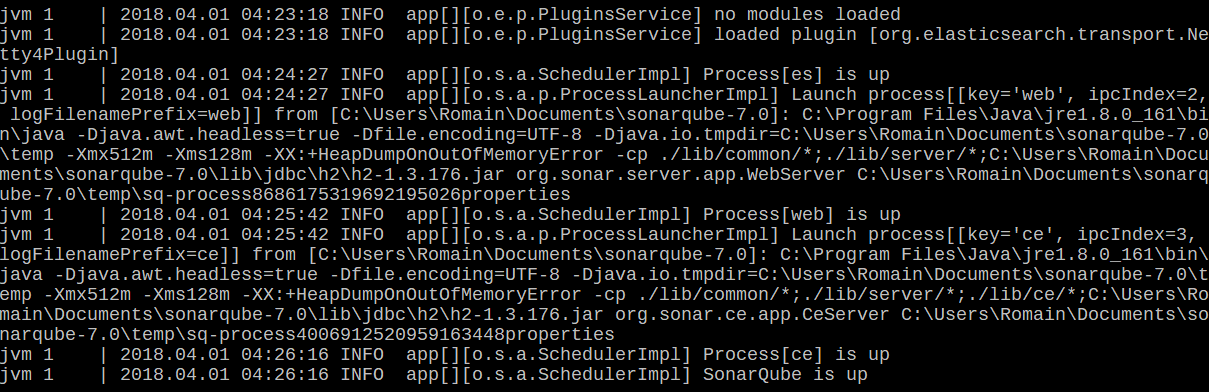
\includegraphics[scale=0.6]{sonarcmd.png}
	\caption{Lancement de l'instance SonarQube}
	\label{fig:sonarcmd}
\end{figure}


Maintenant que SonarQube est opérationnel, nous allons analyser notre projet. Dans un premier temps, nous regarderons l'application Angular. Dans notre cas, on souhaite que Sonar examine les fichiers \textit{typescript}. \'{E}tant donné que nous n'avons pas utilisé d'outils de build pour cette partie, nous avons installé un scanner sonar pour tout type de projet. Pour effectuer une analyse, il suffit de lancer depuis un terminal le script \textit{sonar-scanner} et de créer un fichier \textit{sonar-project.properties} comportant les détails concernant le projet, l'analyse s'effectuera par la suite. Le script va scanner tous les fichiers du dossier depuis lequel nous exécutons le programme et déterminera les éléments à modifier dans le code. Les résultats seront affichés dans l'instance SonarQube sur le navigateur internet.


Lors de notre première analyse sur l'application, nous avons eu les résultats suivants: 

\begin{figure}
	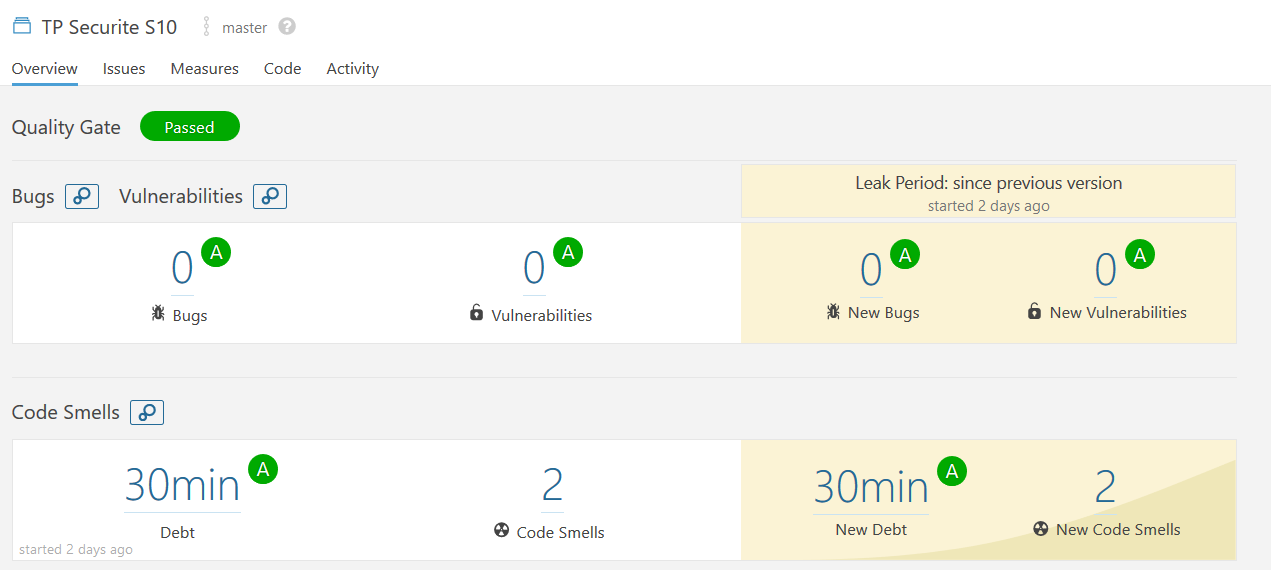
\includegraphics[scale=0.55]{sonarresult.png}
	\caption{Résultats de l'analyse Sonar}
	\label{fig:sonarresult}
\end{figure}

Nous pouvons remarquer que nous avons produit un code sans bug et sans vulnérabilités tout de suite, ce qui est déjà une très bonne chose. Il ne reste ainsi seulement qu'à corriger les deux erreurs détectées par Sonar pour avoir un code qui respecte les règles de Sonar. 


\chapter{Tests de charges}



\chapter*{Bilan et conclusion}


\appendix

\chapter{Interface Humain/Machine}

\chapter{Gestion de projet, diagramme de Gantt}


\chapter{Diagramme de classes}


\chapter{Diagramme de séquences}


\chapter{Guide d'installation et d'utilisation}


\section{Pré-requis}


La plateforme est destinée à fonctionner sur les machines de l’école. Il est nécessaire d'avoir une configuration réseau et matérielle solide si l'on souhaite faire fonctionner un maximum de chaînes en simultané sur l'application. La configuration minimale requise est la suivante :

\begin{itemize}
	\item Windows 7 Pro 64 bits
	\item Intel Xen CPU 3.06GHz
	\item 2 processeurs
	\item 4 Go de RAM
\end{itemize}


Pour la configuration réseau, la plateforme peut fonctionner sur un réseau Wi-Fi domicile mais la charge plafonne autour de 7 streams de qualité moyenne.


\section{Installations}

L'application nécessite plusieurs installations:

\subsection{Streamlink}

Streamlink est le logiciel en Python qui va prendre en charge les streams et qui va activer les flux à lire. Il existe plusieurs moyens de se procurer \textit{streamlink}, le plus simple est l'exécutable disponible à l'adresse : https://github.com/streamlink/streamlink/releases .

L'application fonctionne pour les versions 0.10.0 et supérieurs.

\subsection{VLC}

VLC est le logiciel permettant à l'application de visualiser les chaînes. Le programme  fonctionne avec la version 3.0.1 de VLC disponible à l'adresse suivante : https://get.videolan.org/vlc/3.0.1/win64/vlc-3.0.1-win64.exe


\subsection{Java Runtime Environment}

Le programme est un fichier jar qui fonctionne sur la version 8 de Java. Il est nécessaire pour le faire fonctionner de disposer du JRE 8 disponible à l'adresse : www.oracle.com/technetwork/java/javase/downloads/jre8-downloads-2133155.html


\section{Récupération du projet et fonctionnement}

Le projet se trouve sur le dépôt GitHub disponible à l'adresse suivante : https://github.com/RomainR37/streamPlatform

Une fois sur cette page, vous pouvez soit cloner le dépôt Git sur votre ordinateur, soit télécharger le dossier compressé en cliquant sur le bouton \textit{Clone or download} puis en sélectionnant son choix.

Après avoir récupérer le projet, vous pouvez l'exécuter en lancer une invit de commande Windows (en tapant Win+R au clavier puis \textit{cmd} dans le champ disponible). Une fois sur l'invit, dirigez vous vers le dossier du projet récupéré puis dans le dossier, allez dans le dossier \textit{target}. Il contient le fichier jar exécutable et un fichier texte exemple \textit{testStream.txt}. Pour lancer l'application avec le fichier \textit{testStream.txt} à disposition, la commande est la suivante : \javacode{java -jar streamPlatform-1.0.0-jar-with-dependencies.jar testStream.txt}. L'application se lancera.

\begin{figure}
	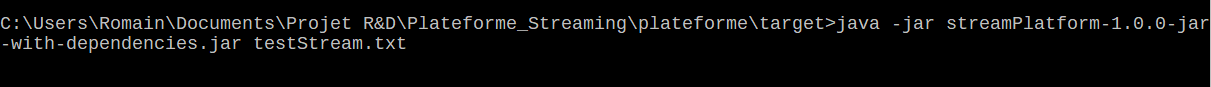
\includegraphics[scale=0.6]{images/cmdLancement.png}
	\caption{Commande de lancement du programme}
\end{figure}


\section{Fichier texte et syntaxe}

Il est possible de lancer l'application avec le fichier texte que l'on souhaite. Celui-ci pour fonctionner devra se situer dans le dossier \textit{target} également. Cependant le fichier doit respecter une convention de nommage. 


Une chaîne nécessite deux informations pour pouvoir fonctionner: son nom et l'adresse du site diffusant son stream. Dans le fichier texte que l'on veut lire, ces deux informations doivent transparaître séparées d'une tabulation. Vous pouvez voir l'exemple du fichier \textit{testStream.txt} ci-après:

\begin{figure}
	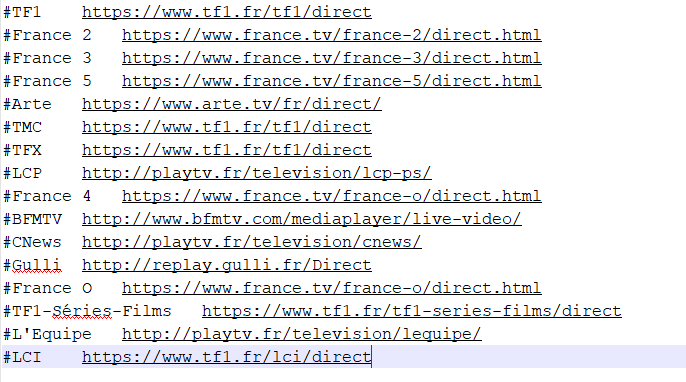
\includegraphics[scale=0.7]{images/testStream.png}
	\caption{Fichier texte exemple \textit{testStream}}
	\label{fig:fichier_texte}
\end{figure}

Ici sur la \autoref{fig:fichier_texte}, nous pouvons voir un \# avant une ligne. Il s'agit de la notation pour mettre une ligne en commentaire. Ainsi, le fichier \textit{testStream.txt} contient déjà une quinzaine de chaînes de télévision fonctionnelles, il suffit donc de supprimer les \# devant la chaîne que l'on veut visualiser. Néanmoins, il est possible de rajouter de nouvelles chaînes tant qu'elle respecte la convention. 

Certaines chaînes ne fonctionnent pas avec streamlink, et ne sont donc pas disponibles sur l'application. Par exemple, la version 0.11.0 de streamlink ne prend pas en charge les chaînes diffusées sur Dailymotion. Le problème sera sans doute réglé dans les prochaines versions ce qui rajoutera de nouvelles chaînes disponibles au visionnage. 


\section{Problèmes pouvant survenir}



\subsection{Pare-feu de Windows}

Un message du firewall peut apparaître au lancement de l'application. Cela est dû au script Python lancé par Streamlink. Il suffit que le firewall accepte les scripts pour que le fonctionnement se passe correctement. 


\subsection{Problèmes d'affichage}

Sur certaines machines, et en particulier sur les machines virtuelles de l'école, il est possible de constater des problèmes d'affichage des chaînes. On peut voir en effet sur des streams de bonne qualité, des problèmes au niveau des contours sur l'image (comme sur la \autoref{fig:pbAffichage}, en particulier à droite de l'image).


\begin{figure}
	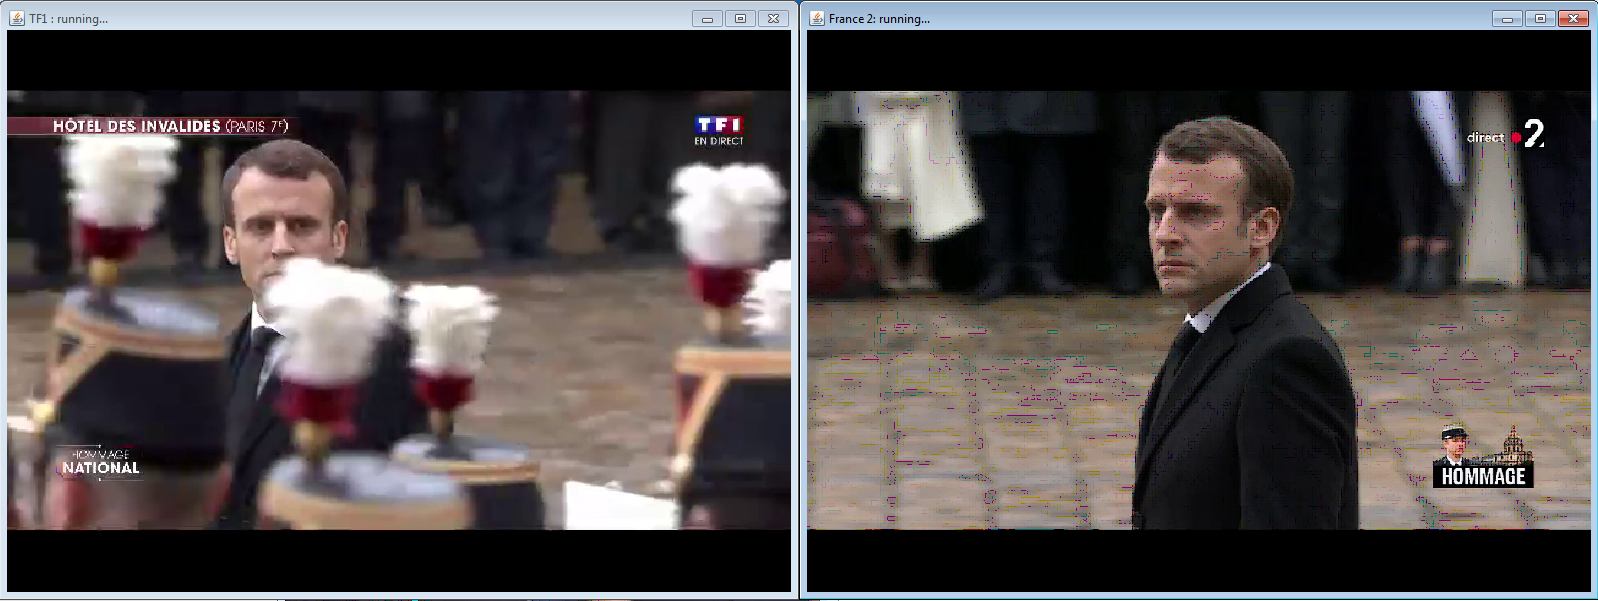
\includegraphics[scale=0.37]{images/imageQualite.png}
	\caption{Exemple de problèmes d'affichage}
	\label{fig:pbAffichage}
\end{figure}


Ces problèmes peuvent venir des configurations graphiques de la machine, notamment de DirectX. Néanmoins, lors des tests effectués sur machines Windows 10, il n'y avait aucun problème d'affichage, donc cela pourrait être des anciens systèmes Windows également.


\end{document}